\documentclass[journal]{IEEEtran}
% Supplementary material for the TCDS article "Private Needs, Shared Rhythms" (main.tex).
% It is not counted in the page limit. Build:
%   pdflatex supplement && bibtex supplement && pdflatex supplement && pdflatex supplement

\usepackage{amsmath,amssymb}
\usepackage{graphicx}
\usepackage{booktabs}
\usepackage{xcolor}
\usepackage{cite}
\usepackage{url}
\usepackage[hidelinks]{hyperref}

% \draftmarkersfalse hides the blue author notes (keep in step with main.tex)
\newif\ifdraftmarkers
\draftmarkerstrue
\newcommand{\authornote}[1]{\ifdraftmarkers\textcolor{blue}{\textit{[Authors: #1]}}\fi}

\newcommand{\eav}{\varepsilon_{Av}}
\newcommand{\eam}{\varepsilon_{Am}}

% everything here is numbered with an S, so that it cannot be confused with the article
\renewcommand{\thesection}{S\arabic{section}}
\renewcommand{\thefigure}{S\arabic{figure}}
\renewcommand{\thetable}{S\arabic{table}}
\renewcommand{\theequation}{S\arabic{equation}}

\begin{document}

\title{Supplementary Material for ``Private Needs, Shared Rhythms: Anchored Partner Models for Attachment-Like Coordination in Robot Dyads''}

\author{Aung~Htet,
        Alejandro~Jimenez-Rodriguez,
        Marcantonio~Gagliardi,
        and~Tony~J.~Prescott}

\markboth{Supplementary material}%
{Htet \MakeLowercase{\textit{et al.}}: Private Needs, Shared Rhythms}

\maketitle

\noindent This document supports the article. Equations (1)--(5), Figs.~1--9 and Table~I refer to the article; equations, figures, tables and sections numbered with an S are in this document. The design names follow the article: the coupled reference (``shared needs'' in figure legends); private models (blind estimate, self-propagated partner model); perceiving, self-propagated; blind, reference; anchored (perceiving estimate, reference partner model); and a perceiving robot with no partner model. Table~\ref{tab:names} maps them to the controller names in the code and data.

% =====================================================================
\section{Training environment and parameters}
\label{sec:training}
The networks were trained in an agent-based strange situation (Table~\ref{tab:params}). Two point agents move in the square $[-1,1]^2$ under the shared-needs dyad, with the fast dynamics $\dot{x}=x-2x^3-y$ and the value $b=0.5$ of~\cite{Htet2024}, integrated with Euler steps of 0.01. The caregiver stays near the centre. The child heads for a randomly chosen corner when $x_c<0$ and approaches the caregiver when $x_c>0$. An agent in approach calls with a probability that decreases with its recent calls, and replies when its partner calls. Each agent keeps a leaky call trace and an evidence trace, which grows when a partner's call follows its own.

The physical network $\Phi_p$ receives the distance between the agents through a 20-step exponential filter, the agent's own $(x,y)$ and $\eam$. The emotional network $\Phi_e$ receives the evidence trace, both agents' calls, the agent's own $(x,y)$ and $\eav$. Separate networks were trained for child and caregiver at ten parameter values spaced evenly in $[0,1]$. The loss was the squared error to the coupling terms of the true needs, plus a penalty on the first and second differences of the output. The training data came from the simulator, apart from one recorded run at $\varepsilon=0$ \authornote{confirm}. The distance filter is implemented as a one-dimensional convolution that weights the oldest of its 20 samples most heavily \authornote{confirm whether this is intended}; the robot controllers reproduce it exactly as trained. In the perceiving designs the robots' distance in metres is scaled by $2/2.61$, the ratio of the widths of the training and Gazebo arenas, and passed through the same filter, and the call and evidence traces are updated at every control tick. The training simulator writes the slow equation as $\dot{y}_c=b\,x_c-\eam\hat\Phi_p-\eav\hat\Phi_e$ (and $+\eam\hat\Phi_p$ for the caregiver) with the targets $\Phi_p=\tfrac12(y_c+y_p)+y_c$ and $\Phi_e=k_0(\tfrac12(y_c-y_p)+y_c+\delta)$; the offset $k_0\delta$ thus enters with the opposite sign from Eq.~(3) of the article, which follows the npj implementation. With this sign the strongly avoidant dyad settles in approach rather than exploration; the estimation results use these targets throughout.

\begin{table}[t]
\centering
\caption{Parameters of the controllers, the training simulator and the networks.}
\label{tab:params}
\footnotesize
\begin{tabular}{@{}ll@{}}
\toprule
Controllers & $a=c=1$, $b=0.7$, $k_0=0.8$, $\delta=0.1$ \\
 & RK4, $h=0.01$ per tick, 30~Hz \\
 & starting needs: identical $(-1,1,-1,1)$, \\
 & \quad or $U(-1,1)$ from the run seed \\
Agent simulator & $\dot{x}=x-2x^3-y$, $b=0.5$, Euler, $\Delta t=0.01$ \\
 & step 0.03, call/evidence decay $0.1$, gain $0.2$ \\
Networks & $\Phi_p$: $4\!\to\!32\!\to\!64\!\to\!32\!\to\!1$, tanh \\
 & $\Phi_e$: $6\!\to\!64\!\to\!128\!\to\!64\!\to\!1$, SiLU \\
Training & 10 parameter values in $[0,1]$, $10^4$ steps each \\
 & 100-step windows, 80/20 split, Adam, lr $5\!\times\!10^{-4}$ \\
 & batch 32, 50 epochs \\
Arena (Gazebo) & $2.61\times2.61$~m, caregiver box $0.3$~m \\
\bottomrule
\end{tabular}
\end{table}

% =====================================================================
\section{The coupled model and the robot controllers' form}
\label{sec:forms}
The article analyses the coupled model in the form of the npj implementation, Eqs.~(1)--(3), and runs the robots with the distance form of the robot controllers, Eq.~(5). In the distance form the coupling terms enter next to the needs of the robot's own copy, and the fast dynamics are twice as fast. In the coupled model, setting $\dot{x}_i=\dot{y}_i=0$ under ambivalence alone gives the inhomogeneous steady state $(\bar x,\bar y,-\bar x,-\bar y)$ with $\bar x^2=(\eam-b)/(2\eam)$ and $\bar y=b\bar x/\eam$, which exists for $\eam>b$; its Jacobian has eigenvalues with positive real part until $\eam\approx0.75$. Under avoidance alone the shared fixed point $(\bar x,\bar y,\bar x,\bar y)$ solves $\bar x^3+\frac{1-q}{2q}\bar x+\frac{\delta}{2}=0$ with $q=k_0\eav/b$; $k_0$ and $\delta$ make the discriminant negative for every $\eav\in[0,1]$, so the root is unique, and it becomes stable at $\eav\approx0.69$, with $\bar x<0$ (exploration).

Fig.~\ref{fig:forms} repeats the analysis of Fig.~2 of the article for the distance form with the coupling terms of the true needs (the coupled reference). From random starts it synchronises under avoidance and anti-synchronises under ambivalence from weak coupling on, at $\pm1.00$, and slows as the coupling grows; but instead of settling it escapes, from $\eav=0.24$ and $\eam=0.44$, and 95\% of the plane escapes. The two forms therefore agree on the phase relations of the oscillatory regimes and differ at strong coupling and at weak ambivalence, where the coupled model starts synchronised. Over the plane from random starts (Fig.~\ref{fig:maps}), private models in the distance form oscillate with a median $|r|$ of 0.05 where the coupled reference reaches 1.00.

The escape at high avoidance has a simple origin. In the symmetric state $y_c=y_p=y$, Eq.~(5) with the controllers' coupling terms, $d_p=\tfrac12(y_c+y_p)+y_c$ and $d_e=k_0(\tfrac12(y_c-y_p)+y_c+\delta)$, reduces to $\dot{y}=b'x+\eav k_0 (y+\delta)$, so avoidance feeds the accumulated need back on itself with gain $\eav k_0$. For large $|y|$ the need follows the outer branch of the slow manifold, where $x\approx-(y/4)^{1/3}$, and the restoring drift $b'x$ grows only as $|y|^{1/3}$. The accumulated need therefore escapes once its excursion exceeds
\begin{equation}
y^*(\eav) = \left(\frac{b'}{\eav k_0\, 4^{1/3}}\right)^{3/2},
\end{equation}
which falls from 1.62 at $\eav=0.4$ to 1.09 at $\eav=0.52$. From the identical start the shared-needs dyad escapes from $\eav=0.52$. Random starts, whose excursions can be larger, escape from $\eav=0.24$ on in a growing fraction of runs.


\begin{figure*}[t]
\centering
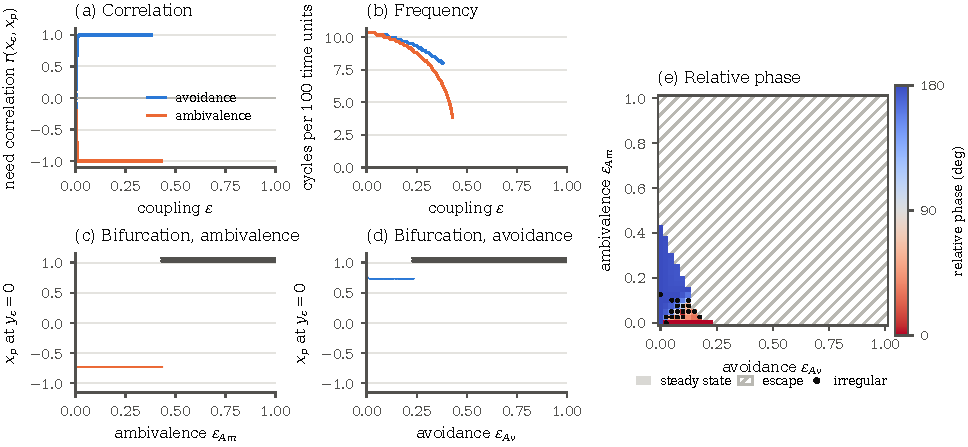
\includegraphics[width=\textwidth]{figures/fig_canonical_distance.pdf}
\caption{The analysis of Fig.~2 of the article repeated for the distance form of the robot controllers with the coupling terms of the true needs. Panels as in Fig.~2; hatched: escape.}
\label{fig:forms}
\end{figure*}

\begin{figure*}[t]
\centering
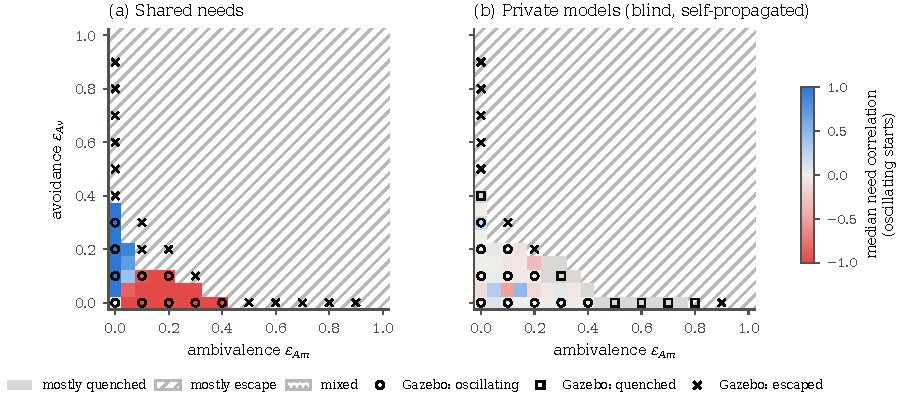
\includegraphics[width=0.8\textwidth]{figures/fig_maps.pdf}
\caption{Regimes over the avoidance--ambivalence plane from random starting needs (20 per cell, 200 model time units). Colour: median coordination where at least half the starts oscillate. Grey: mostly quenched; hatched: mostly escape; dotted: mixed. Markers: majority regime of the Gazebo runs from random starts at each parameter pair.}
\label{fig:maps}
\end{figure*}

% =====================================================================
\section{Simulated strange situation}
\label{sec:sim}
The simulated SSP uses the agent-based simulator in which the networks were trained, with the coupled model of the article (the sign of Eq.~(3)), 10,000 steps per regime and a time constant of one. The caregiver is held near a central base; the child heads for a randomly chosen corner when its need is negative and for the base when it is positive; an agent in approach calls with a probability that decreases with its recent calls and replies to its partner. The time near the caregiver is the fraction of steps with the child inside the square of half the room's width around the caregiver. Across the five regimes it was 50\%, 38\%, 18\%, 53\% and 100\% (secure, moderately and strongly avoidant, moderately and strongly ambivalent), $\chi^2=14{,}676$ with 4 degrees of freedom and $N=50{,}000$. Bonferroni-corrected $z$-tests separated every pair ($p<0.05$); the closest pair, secure and moderately ambivalent, differed at $p=0.011$. The correlation of the needs was 0.39 (secure), 0.66 and 0.96 (avoidant) and $-0.84$ and $-0.54$ (ambivalent). The npj draft reported 52\%, 41\%, 18\%, 52\% and 99.9\% for the same procedure.

% =====================================================================
\section{Physical-robot strange situation}
\label{sec:physical}
These experiments, reported in the npj draft, ran the coupled model on two MiRo-e robots (Fig.~\ref{fig:robotsetup}). The caregiver sat on a box surrounded by AprilTags, which the child approached; the robots exchanged calls with MiRo's vocal synthesiser, accumulating evidence of a completed exchange with a drift-diffusion process, and the child was tracked with an overhead camera. Physical and emotional distance were measured from the robots' positions and vocal exchange and modulated a coupling that still read both needs. Periods in which the exploring child was stuck at a wall (longer than the mean plus two standard deviations in one cell of a $50\times50$ grid) were excluded. The child spent 54\% of the time near the caregiver in the secure regime ($\eam=0.1$), 41\% in the strongly avoidant regime ($\eav=0.9$) and 43\% in the moderately ambivalent regime ($\eam=0.4$), $\chi^2=99.38$ with 2 degrees of freedom and $N=29{,}743$; Bonferroni-corrected tests separated the secure regime from both others but not the avoidant from the ambivalent one (Figs.~\ref{fig:robotruns}--\ref{fig:robotheat}). The ambivalent robot spent more time away from the caregiver than the simulation predicted, and the avoidant robot kept some oscillation where the model predicts a fixed point. \authornote{these numbers and figures are taken from the npj draft; the recordings are not in the repository}

\begin{figure}[t]
\centering
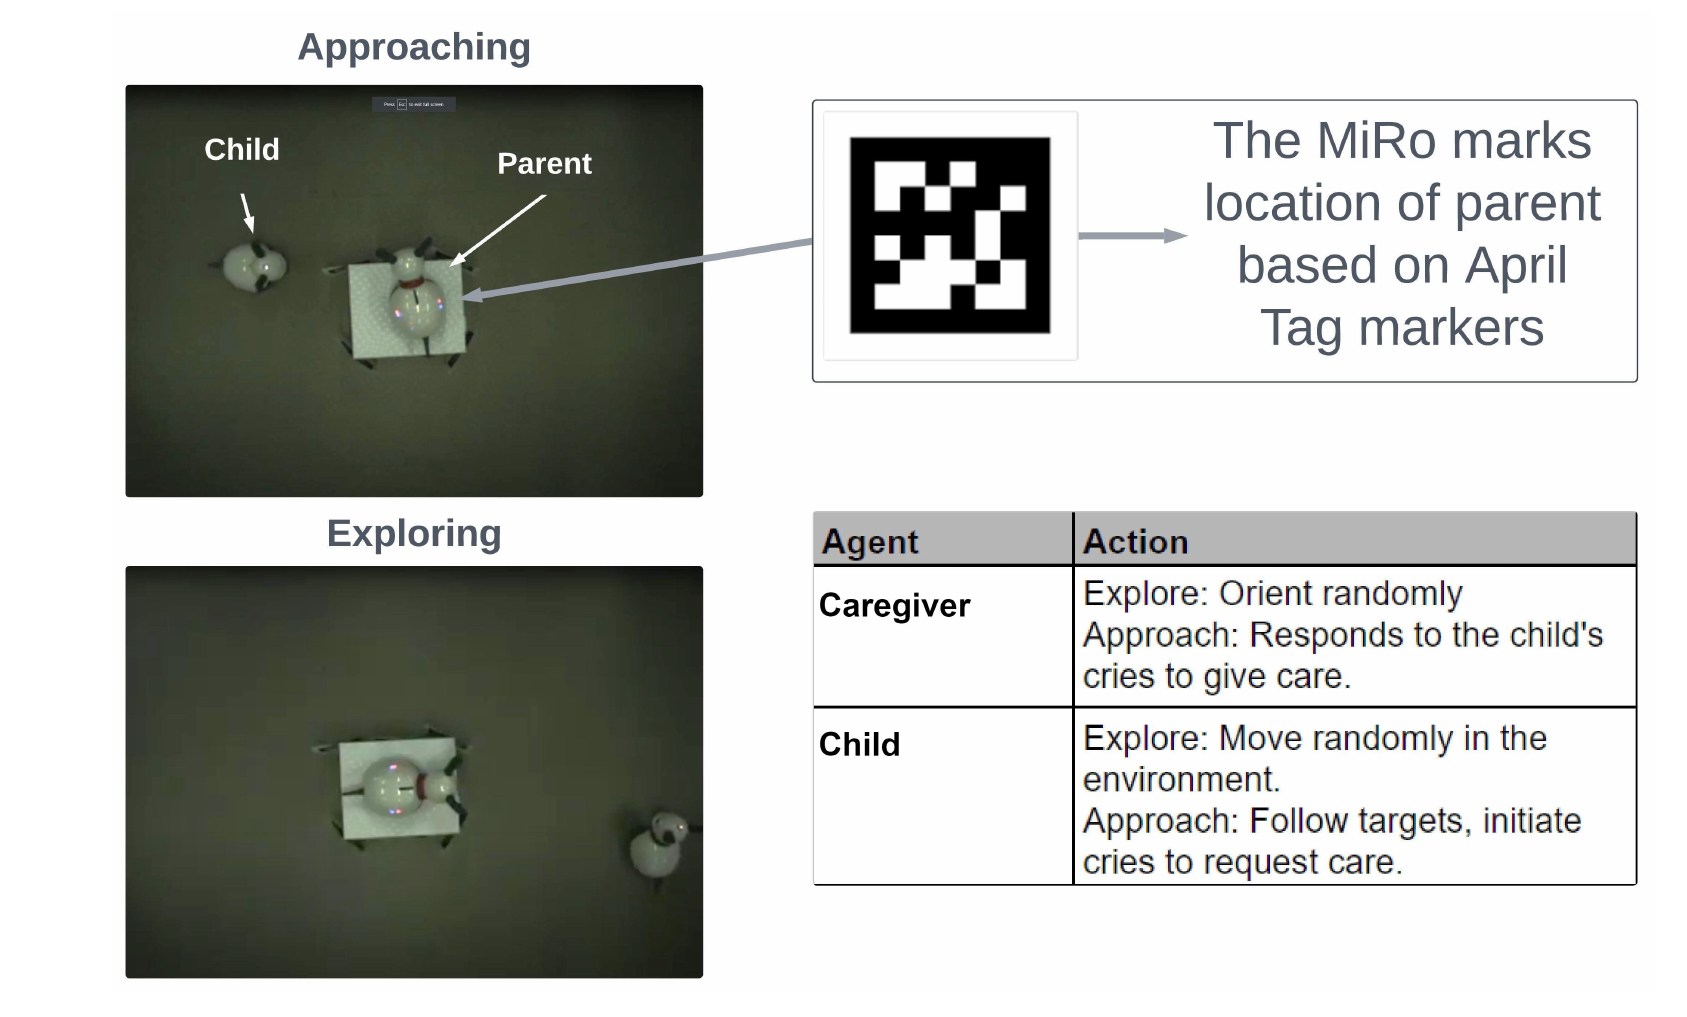
\includegraphics[width=\columnwidth]{figures/npj_robot_setup.png}
\caption{The physical-robot SSP: the arena with the caregiver on its box and the child, approaching (top) and exploring (bottom), the AprilTag markers and the robots' actions (from the npj draft).}
\label{fig:robotsetup}
\end{figure}

\begin{figure}[t]
\centering
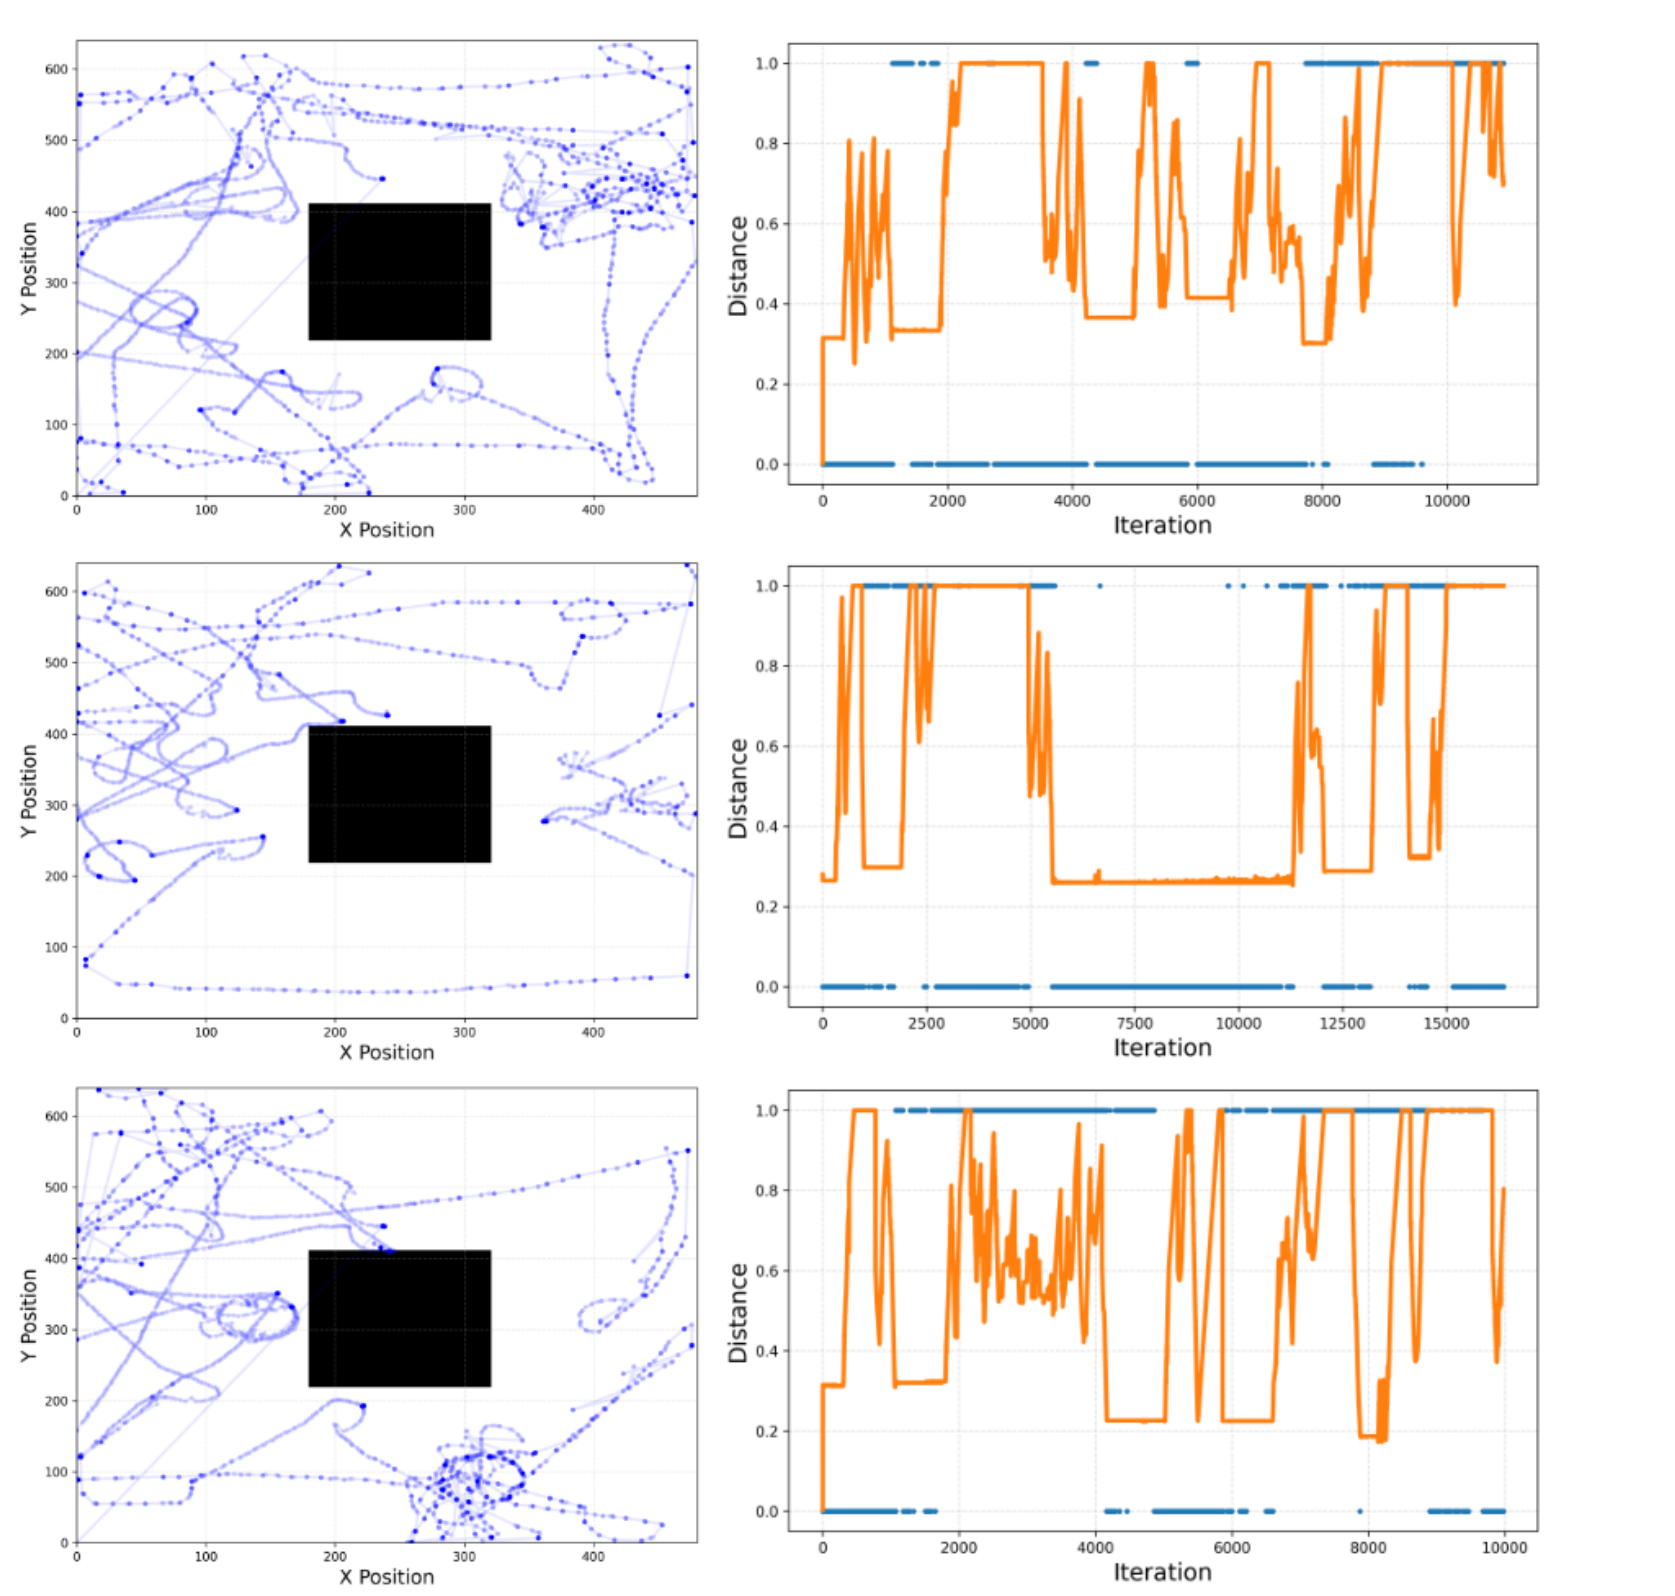
\includegraphics[width=\columnwidth]{figures/npj_robot_runs.png}
\caption{Physical robots: the child's path relative to the caregiver (left) and the normalised distance from the centre with the child's calls (right) in the secure ($\eam=0.1$, top), strongly avoidant ($\eav=0.9$, middle) and moderately ambivalent ($\eam=0.4$, bottom) regimes (from the npj draft).}
\label{fig:robotruns}
\end{figure}

\begin{figure}[t]
\centering
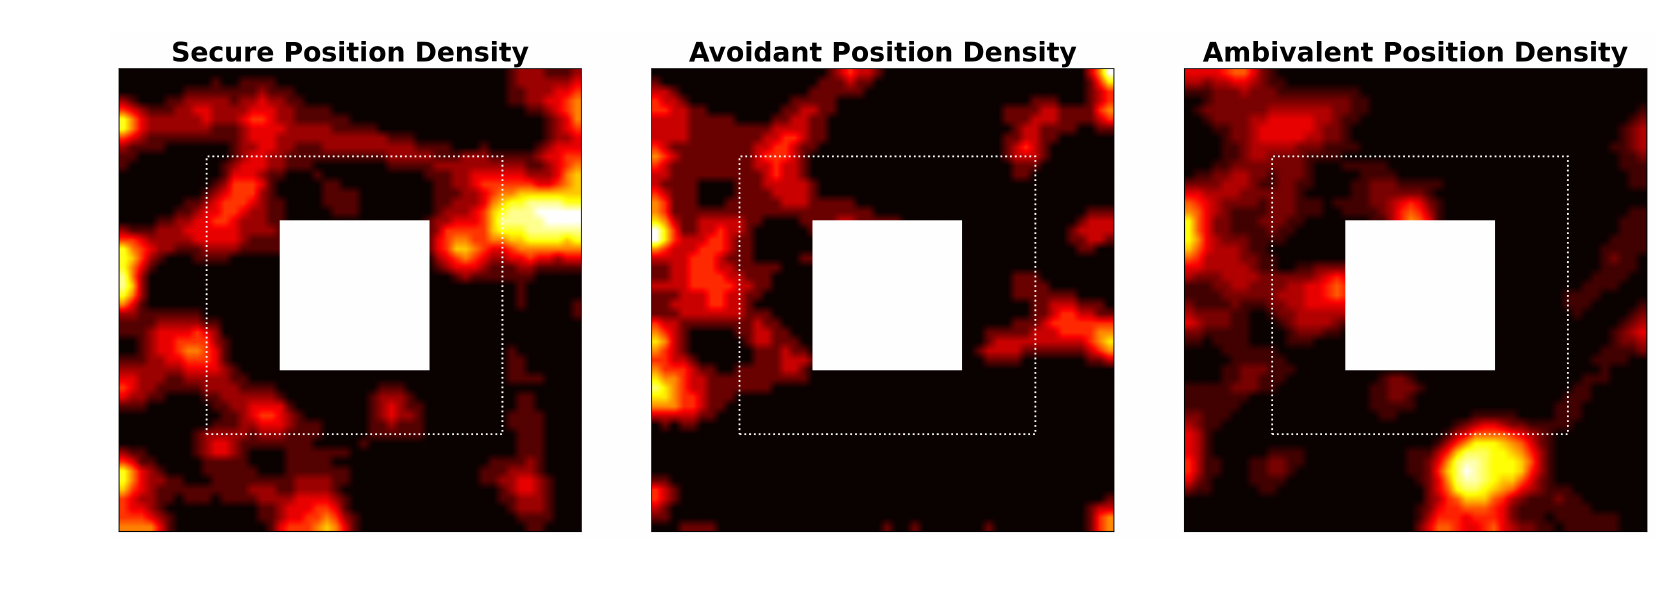
\includegraphics[width=\columnwidth]{figures/npj_robot_heatmaps.png}
\caption{Physical robots: where the child spent its time on a $50\times50$ grid, stuck periods removed, in the secure, avoidant and ambivalent regimes (from the npj draft).}
\label{fig:robotheat}
\end{figure}

% =====================================================================
\section{The learned estimates}
\label{sec:estimates}

\subsection{Offline accuracy}
Fed the inputs of analytically coupled runs in the agent simulator, the networks reproduce the coupling closely (Fig.~\ref{fig:estimator}a). For $\varepsilon\geq0.1$ the median root-mean-square error is 0.028 and 0.037 for the child's and caregiver's physical networks, and 0.041 and 0.014 for their emotional networks, in units in which the coupling varies by about two over a cycle; accuracy is comparable at held-out parameter values. Removing inputs shows what the estimates rely on (Fig.~\ref{fig:estimator}b). The physical estimate rests mainly on the agent's own need: without it the median $R^2$ falls to 0.26 and 0.44, from 0.98 with all inputs. The distance acts as a correction, with $R^2$ of 0.98 and 0.80 without it. The emotional estimate needs the vocal exchange: with the calls silenced, as in the blind designs, $R^2$ falls to 0.63 for the child and to $-0.12$ for the caregiver. In closed loop in the simulator, with the learned estimate replacing the analytic coupling in both agents, the anti-synchrony of the analytic dyad is replaced by weak correlations (Fig.~\ref{fig:estimator}c,d).

\begin{figure*}[t]
\centering
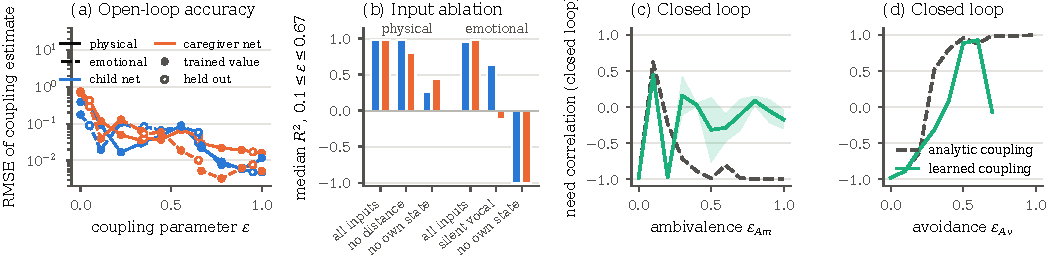
\includegraphics[width=\textwidth]{figures/fig_estimator.pdf}
\caption{The learned estimates in the agent simulator. (a) Open-loop error of the four networks against the analytic coupling, at the training values (filled) and at held-out values (open). (b) Median $R^2$ for $0.1\leq\varepsilon\leq0.67$ when one input group is removed: the distance (physical networks), the calls, silenced as in the blind designs (emotional networks), or the agent's own need. (c,d) Coordination in closed loop with analytic or learned coupling (mean $\pm$ s.d., 10 seeds).}
\label{fig:estimator}
\end{figure*}

\subsection{Estimation on the robots by design}
Table~\ref{tab:estimation} and Fig.~\ref{fig:estimation} summarise the learned estimates on the robots. When the child hears the calls, its emotional estimate follows the coupling of the true needs with a correlation of 0.96--0.97 under avoidance. With silent calls it is inverted under avoidance, at $-0.51$ with a self-propagated and $-0.80$ with a reference partner model, which is why the blind private model believes in anti-synchrony under avoidance. Under ambivalence the child's estimate follows the coupling in every design (0.80--0.87). The caregiver's estimate is poor in every design, with correlations between $-0.48$ and 0.27, so the two roles are not symmetric. Only the anchored design's partner model tracks the caregiver (Fig.~\ref{fig:estimation}c,d). Perception and a reference partner model both make the avoidant dyad less stable: across the avoidance strip, 85--89\% of their runs escape, against 58\% for the blind private model.

\begin{table}[t]
\centering
\caption{Estimation on the robots by design, named by perception and partner model (Gazebo, random starts, $\varepsilon>0$, along the avoidance (Av) and ambivalence (Am) strips). Escaped: fraction of runs; estimates and tracking: means over runs that did not escape. Estimates are correlated with the coupling computed from both robots' true needs; partner tracking compares the child's model of the caregiver with the caregiver's own need.}
\label{tab:estimation}
\footnotesize
\setlength{\tabcolsep}{3pt}
\resizebox{\columnwidth}{!}{\begin{tabular}{@{}lcccccccc@{}}
\toprule
 & \multicolumn{2}{c}{Escaped} & \multicolumn{2}{c}{Child estimate $r$} & \multicolumn{2}{c}{Caregiver estimate $r$} & \multicolumn{2}{c}{Partner tracking $r$} \\
\cmidrule(lr){2-3}\cmidrule(lr){4-5}\cmidrule(lr){6-7}\cmidrule(l){8-9}
Design & Av & Am & Av & Am & Av & Am & Av & Am \\
\midrule
blind / self & 58\% & 16\% & $-0.51$ & $+0.80$ & $-0.08$ & $+0.13$ & $+0.27$ & $+0.16$ \\
perceiving / self & 85\% & 11\% & $+0.96$ & $+0.84$ & $+0.12$ & $-0.11$ & $+0.48$ & $+0.09$ \\
perceiving (odometry) / self & 85\% & 11\% & $+0.96$ & $+0.84$ & $+0.11$ & $-0.18$ & $+0.42$ & $+0.11$ \\
blind / reference & 85\% & 44\% & $-0.80$ & $+0.83$ & $+0.00$ & $+0.08$ & $+0.28$ & $+0.11$ \\
perceiving / reference & 89\% & 44\% & $+0.97$ & $+0.87$ & $+0.26$ & $-0.48$ & $+0.79$ & $+0.64$ \\
no partner model & 0\% & 11\% & $+0.71$ & $+0.79$ & $+0.14$ & $+0.27$ & --- & --- \\
\bottomrule
\end{tabular}
}
\end{table}

\begin{figure*}[t]
\centering
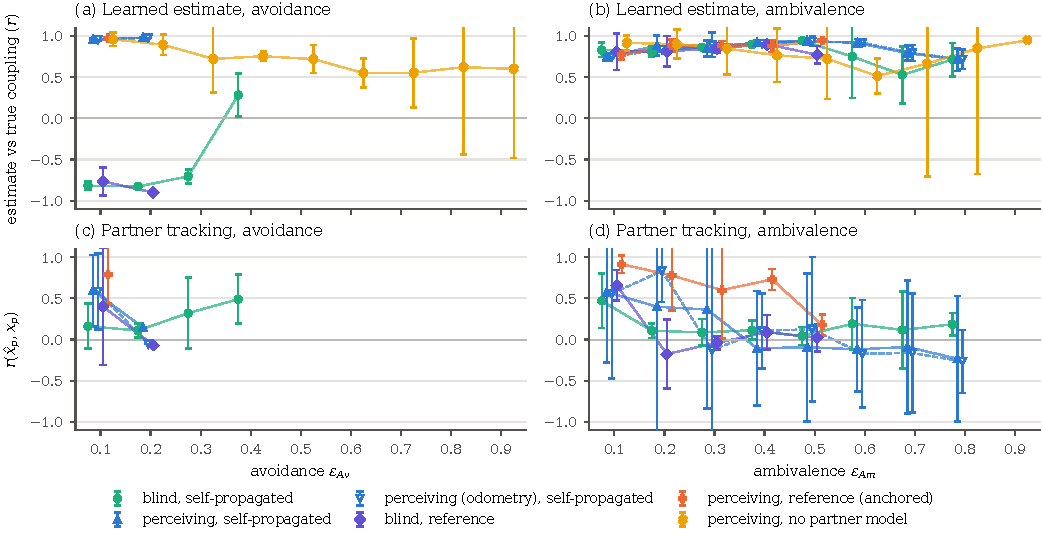
\includegraphics[width=\textwidth]{figures/fig_estimation.pdf}
\caption{Estimation and partner tracking on the robots, by design (Gazebo, random starts, mean and 95\% interval over three seeds, or five for the blind, self-propagated design; runs that escaped are omitted). (a,b) Correlation between the child's learned estimate and the coupling terms computed from both robots' true needs. (c,d) Partner tracking: the child's model of the caregiver against the caregiver's own need.}
\label{fig:estimation}
\end{figure*}

\subsection{Belief and coordination after transients}
Over 300 model time units with the first 100 discarded, the median coordination of private models lies within 0.11 of zero for every $\varepsilon$ from 0.1 to 0.4 on both strips, while the child's belief stays anti-synchronised under ambivalence and the partner model does not follow the partner (Fig.~\ref{fig:belief}). At $\eam=0.2$ the child's need runs at 24.8~mHz and the caregiver's at 31.5~mHz; with shared needs both run at 27.8~mHz.

\begin{figure*}[t]
\centering
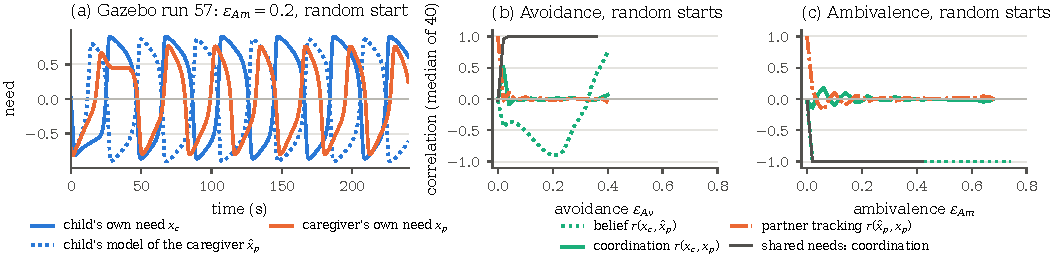
\includegraphics[width=\textwidth]{figures/fig_belief.pdf}
\caption{Belief and reality with private models. (a) Controller logs of a Gazebo run at $\eam=0.2$ from random starting needs. (b,c) After transients (median of 40 random starts): the child's belief, the coordination of the two robots' needs, partner tracking, and the coordination of the shared-needs dyad.}
\label{fig:belief}
\end{figure*}

\subsection{Assignment of networks}
In the blind designs both robots use the networks trained on the caregiver's data, as in the original controller, and in the perceiving designs each robot uses its own networks \authornote{confirm this assignment}. The loss of coordination with private models does not depend on this. When each robot uses its own networks, the belief under avoidance becomes synchronised, but coordination after transients remains near zero at $\eav=0.1$ (0.01) and at $\eam=0.2$ (0.00); some anti-synchrony survives only at $\eam=0.1$ ($-0.68$).

\subsection{A robot without a partner model}
Without a partner model, a perceiving robot integrates only its own need, with the equations of the training simulator, and takes the whole coupling term from its networks. Its estimate follows the coupling of the true needs with correlations of 0.71 under avoidance and 0.79 under ambivalence, and its needs never escape along the avoidance strip. Its need, however, shows no consistent phase relation with the caregiver's, with mean coordination between $-0.03$ and 0.51 for $0.1\leq\eam\leq0.4$ and standard deviations up to 0.96 over runs.

% =====================================================================
\section{Robot behaviour}
\label{sec:behaviour}

\subsection{Arena and behaviours}
The Gazebo arena is shown in Fig.~\ref{fig:arena}. When exploring, the child drives at a commanded 0.2~m/s (about 0.12~m/s realised), redraws a random turn rate during even-numbered seconds, and turns in place when its sonar reads less than 0.105~m. When approaching, it steers towards a tag seen in either camera, stops when the sonar reads less than 0.2~m, and rotates in search when no tag is visible. The child calls while it approaches with a tag in view, and the caregiver calls while its own need is in approach. Each robot's controller runs as a separate thread and logs its full working model, its network inputs and its coupling estimates at every tick; needs, actions, calls, wheel odometry and ground-truth positions were recorded at 10~Hz, together with an overhead video.

\begin{figure}[t]
\centering
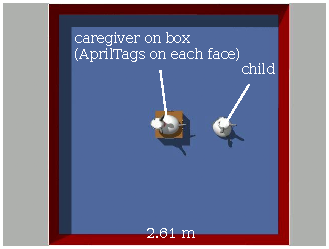
\includegraphics[width=0.8\columnwidth]{figures/fig_arena.pdf}
\caption{The Gazebo arena seen by the overhead camera, with the caregiver on its box at the centre and the child beside it.}
\label{fig:arena}
\end{figure}

\subsection{Behaviour at three conditions}
Table~\ref{tab:conditions} compares shared needs and private models at three conditions. \emph{Time near the caregiver} is the fraction of samples with the child inside the central square of half the arena's width~\cite{Htet2024}, excluding periods in which the exploring child was stuck against a wall (a median of 8\% of a run). Time near the caregiver and calling rates separate the regimes less well than call reciprocity within a 180~s run; they mainly mark the transitions to quenching and escape, such as the caregiver's silence at strong ambivalence and the child's settling beside the box when its need is fixed in approach (Fig.~\ref{fig:regimes}, bottom).

\begin{table*}[t]
\centering
\caption{Behaviour with shared needs and with private models in Gazebo at three conditions (random starts, first 180~s, mean $\pm$ s.d. over runs; coordination omits runs that escaped).}
\label{tab:conditions}
\footnotesize
\begin{tabular}{@{}llcccccc@{}}
\toprule
$(\varepsilon_{Av},\varepsilon_{Am})$ & Design & $n$ & $r(x_c,x_p)$ & Near (\%) & Child calls (\%) & Carer calls (\%) & Reciprocity \\
\midrule
(0.2, 0) & shared needs & 3 & $0.94 \pm 0.04$ & $60 \pm 10$ & $17 \pm 6$ & $52 \pm 4$ & $1.00 \pm 0.00$ \\
(0.2, 0) & private models & 5 & $0.07 \pm 0.15$ & $58 \pm 7$ & $22 \pm 4$ & $53 \pm 4$ & $0.60 \pm 0.15$ \\
(0, 0.2) & shared needs & 3 & $-0.95 \pm 0.07$ & $46 \pm 17$ & $18 \pm 7$ & $48 \pm 5$ & $0.29 \pm 0.12$ \\
(0, 0.2) & private models & 5 & $-0.04 \pm 0.12$ & $57 \pm 10$ & $18 \pm 6$ & $48 \pm 3$ & $0.65 \pm 0.14$ \\
(0, 0.7) & shared needs & 3 & --- & $78 \pm 23$ & $5 \pm 4$ & $62 \pm 33$ & $0.39 \pm 0.53$ \\
(0, 0.7) & private models & 5 & $-0.03 \pm 0.51$ & $75 \pm 30$ & $2 \pm 2$ & $62 \pm 41$ & $0.84 \pm 0.27$ \\
\bottomrule
\end{tabular}

\end{table*}

\begin{figure*}[t]
\centering
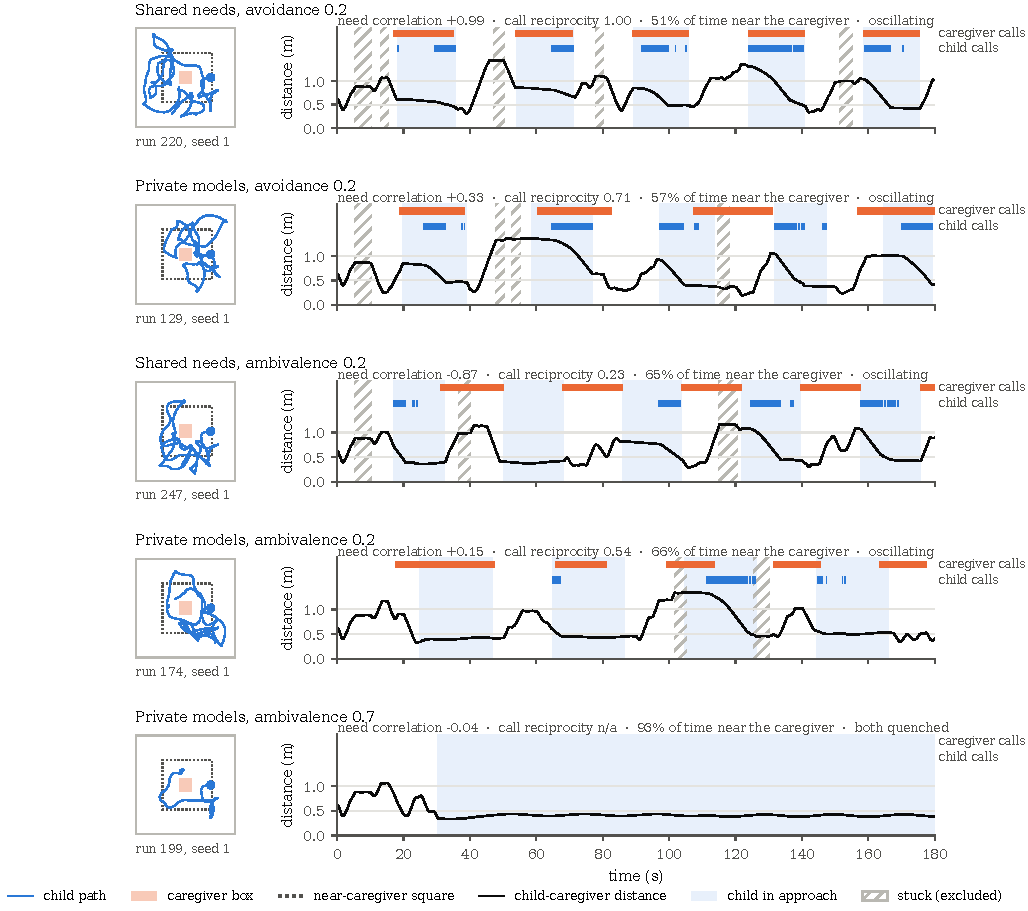
\includegraphics[width=\textwidth]{figures/fig_gazebo_regimes.pdf}
\caption{Gazebo runs with shared needs and with private models from the same random starting needs (seed 1), including a run at $\eam=0.7$ in which both needs are quenched. Left: the child's path (blue), the caregiver's box (orange) and the near-caregiver square (dotted). Right: the distance between the robots, periods with the child in approach (shaded), periods in which the child was stuck (hatched) and the calls of the child and caregiver (bars), over the first 180~s.}
\label{fig:regimes}
\end{figure*}

\subsection{Fifteen-minute runs}
Over 15 minutes the shared-needs dyad holds its behavioural signature (Fig.~\ref{fig:long}). Its caregiver answers almost every call under avoidance and, in 120~s windows, between 3\% and 47\% of them under ambivalence, with the needs at $r=1.00$ and $-1.00$. With private models, reciprocity wanders between 0.18 and 1.00 as the two working models drift in and out of phase, and the coordination of the needs oscillates around zero. A coordinated dyad is thus distinguished not only by its average responsiveness but by its steadiness.

\begin{figure*}[t]
\centering
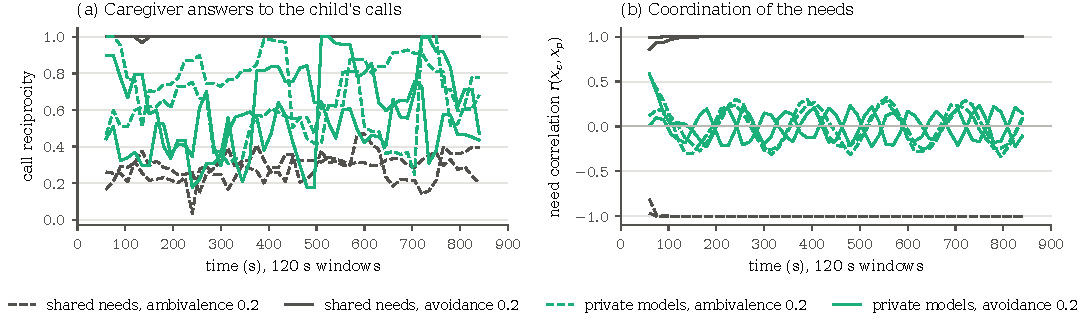
\includegraphics[width=\textwidth]{figures/fig_long.pdf}
\caption{Fifteen-minute Gazebo runs from random starting needs (two seeds per condition), in sliding 120~s windows. (a) Fraction of the child's calling time answered by the caregiver. (b) Coordination of the two robots' needs.}
\label{fig:long}
\end{figure*}

\subsection{Sweeps and the kinematic stand-in}
\label{sec:standin}
To generate the many runs the observers of Section~\ref{sec:inverse} need, we built a kinematic stand-in for the Gazebo experiment. It reproduces the arena, box and starting pose of the Gazebo world and the child's behaviours at 10~Hz, driven by the private-model controller. It uses a unicycle model, a sonar ray cast to the walls and the box, and cameras covering bearings from $-15^\circ$ to $60^\circ$ (left) and the mirror image (right). Tags are visible between 0.5~m and 1.9~m from the box centre; the near limit reproduces the child's loss of the tags beside the box. When the controller's needs escape, the last value before the first undefined value persists, as in the robot controller. The exploration speed was set to 0.12~m/s, the value that best matched the Gazebo runs over a grid from 0.10 to 0.20~m/s. Because the needs of private models do not depend on behaviour, the stand-in follows the robots' sequence of approach and exploration exactly, and with this speed it also matches their behaviour across the sweeps (Fig.~\ref{fig:sweeps}).

\begin{figure*}[t]
\centering
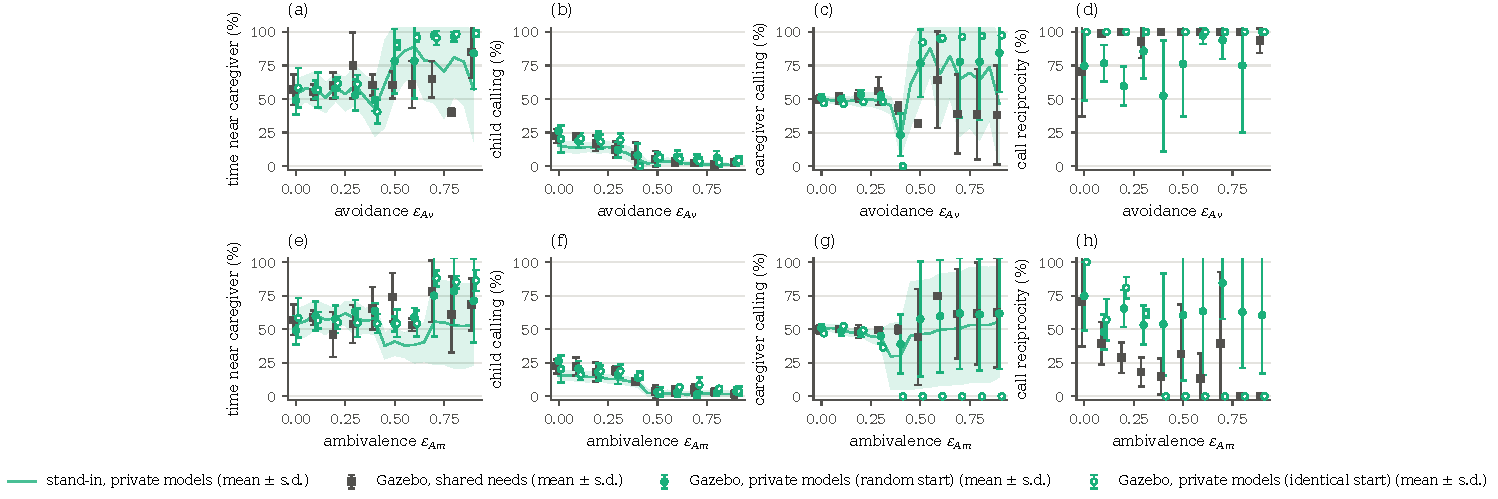
\includegraphics[width=\textwidth]{figures/fig_gazebo_sweeps.pdf}
\caption{Behaviour across the Gazebo sweeps with shared needs (grey squares) and private models from random (filled circles) and identical (open circles) starts, mean $\pm$ s.d. over runs. Band: the kinematic stand-in driven by private models from random starts (30 seeds, mean $\pm$ s.d.).}
\label{fig:sweeps}
\end{figure*}

\subsection{Wheel odometry}
Wheel odometry drifted by a median of 1.06~m over a 180~s run, about 40\% of the arena's width (Fig.~\ref{fig:odometry}), so positions are taken from ground truth. The perceiving, self-propagated design run with odometry distances estimated the coupling as well as with ground truth (Table~\ref{tab:estimation}), consistent with the physical estimate's reliance on the robot's own need rather than on the distance (Section~\ref{sec:estimates}).

\begin{figure}[t]
\centering
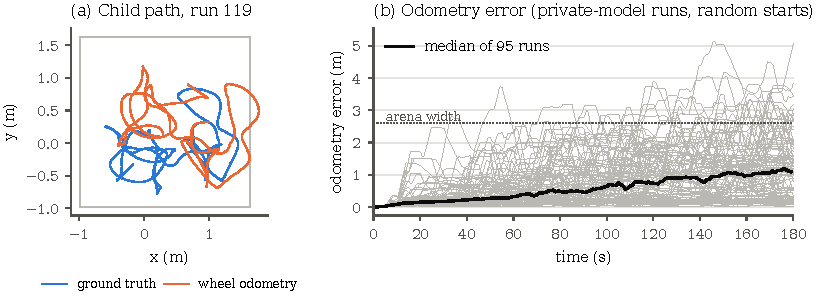
\includegraphics[width=\columnwidth]{figures/fig_odometry.pdf}
\caption{Wheel odometry against ground truth in the Gazebo runs. (a) The child's path in one run. (b) Odometry error over time in the 95 runs of private models from random starts.}
\label{fig:odometry}
\end{figure}

% =====================================================================
\section{Reading parameters from behaviour}
\label{sec:inverse}
The training set comprised 1110 stand-in runs of 180~s, covering both strips from 0 to 0.9 in steps of 0.05 with 30 seeds each, 10 from the identical start and 20 from random starts. Runs were labelled secure ($\varepsilon\leq0.1$), avoidant or ambivalent. The observer of the child used the time near the caregiver, the mean and standard deviation of the distance, the fraction of time calling and the rate of distance cycles; the observer of the dyad added the caregiver's calling fraction and call-bout rate. Both were random forests with 400 trees. The test set comprised the 176 Gazebo runs of private models on the strips, 99 of them from random starts. The child-only observer mistook many mild avoidant and ambivalent runs for secure ones (Fig.~\ref{fig:inverse}a). In the dyad observer, the caregiver's calling fraction and call-bout rate carry half of the feature importance. Trained on the Gazebo runs themselves, with far fewer runs to learn from, the two observers reached 56\% and 74\%.

\begin{figure*}[t]
\centering
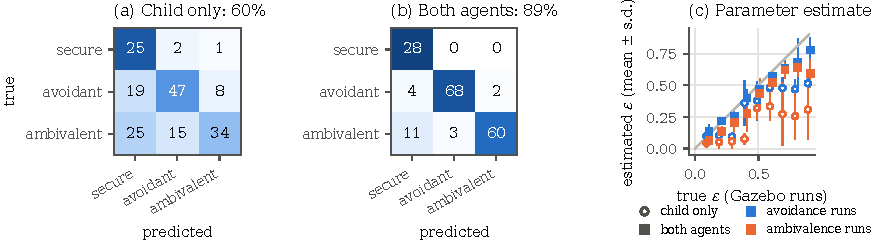
\includegraphics[width=0.85\textwidth]{figures/fig_inverse.pdf}
\caption{Reading the attachment parameters from behaviour in the 176 Gazebo runs of private models, with observers trained only on the kinematic stand-in. (a,b) Regime classification by an observer of the child and an observer of both robots. (c) Estimated against true parameter, mean $\pm$ s.d. over runs, for avoidance (blue) and ambivalence (orange) runs.}
\label{fig:inverse}
\end{figure*}

% =====================================================================
\section{Runs, validation and code names}
\label{sec:runs}
We recorded 577 Gazebo runs (Table~\ref{tab:names}), six at a time in separate containers, with a median real-time factor of 0.97 (minimum 0.76). Runs lasted 180~s, apart from eight runs of 900~s and some of the 20 earliest runs, which lasted up to 300~s. Along both strips, at $(0,0)$ and at $\varepsilon=0.1,\dots,0.9$, private models were run from five random starts and from the identical start, shared needs from three random starts and the identical start, and the other four designs from three random starts; the perceiving, self-propagated design was run once with ground-truth and once with odometry distances. Six off-axis points were run with shared needs and with private models. Random starts were drawn from seeds 1--5, so a given seed gave the same starting needs in every condition and design.

Each run was checked against its controller. With shared needs and in the blind designs the needs do not depend on behaviour, so integrating the controller offline from the run's logged starting needs must reproduce them. It did, with a correlation above 0.999 in every bounded run, and it escaped in exactly the runs whose needs escaped. In the perceiving designs behaviour feeds back into the needs, so we checked instead that the inputs each controller logged match what the robots recorded: the distance matched within 0.1~cm, and the calls matched the robots' calls in at least 96\% of samples. All 557 logged runs passed, and the 20 earliest runs, which predate the controller logs, were replayed against their recorded needs.

\begin{table}[t]
\centering
\caption{Design names, the corresponding controller settings in the code, and the number of Gazebo runs.}
\label{tab:names}
\footnotesize
\setlength{\tabcolsep}{3pt}
\begin{tabular}{@{}llr@{}}
\toprule
Design & \texttt{controller}, \texttt{distance} & Runs \\
\midrule
Shared needs & \texttt{coupled} & 98$^a$ \\
Blind, self-propagated$^b$ & \texttt{decoupled} & 194\phantom{$^a$} \\
Perceiving, self-propagated & \texttt{observed}, \texttt{gt} & 57\phantom{$^a$} \\
 & \texttt{observed}, \texttt{odom} & 57\phantom{$^a$} \\
Blind, reference & \texttt{baseline} & 57\phantom{$^a$} \\
Perceiving, reference (anchored) & \texttt{baseline-observed}, \texttt{gt} & 57\phantom{$^a$} \\
Perceiving, no partner model & \texttt{notebook}, \texttt{gt} & 57\phantom{$^a$} \\
\midrule
Total & & 577\phantom{$^a$} \\
\bottomrule
\multicolumn{3}{@{}p{0.95\columnwidth}@{}}{\scriptsize $^a$19 from the identical start. $^b$Called private models in the article; 77 runs from the identical start. All other runs start from random needs.}
\end{tabular}
\end{table}

\bibliographystyle{IEEEtran}
\bibliography{refs}

\end{document}
